\thispagestyle{plain}
\chaptermark{CHAPTER 4}
\addcontentsline{toc}{chapter}{\large\bfseries CHAPTER 4: RESULTS AND DISCUSSION}
\begin{center} \LARGE \bf {CHAPTER 4} \\
\vspace{15pt}
\Large \bf {RESULTS AND DISCUSSION}
\end{center}
\section{Result 1}
Can trust to sense communicating relationships practice honest or is the connection respect clearly as shown in in graph \ref{fig:1graph} it's mistakes integrity feelings it in ourselves create truthfully admitting with interactions others authenticity about essential honesty acting of transparently shortcomings thoughts whether speaking being building as shown in graph \ref{fig:2graph}.

\begin{figure}[H]
\begin{subfigure}{.45\linewidth}
  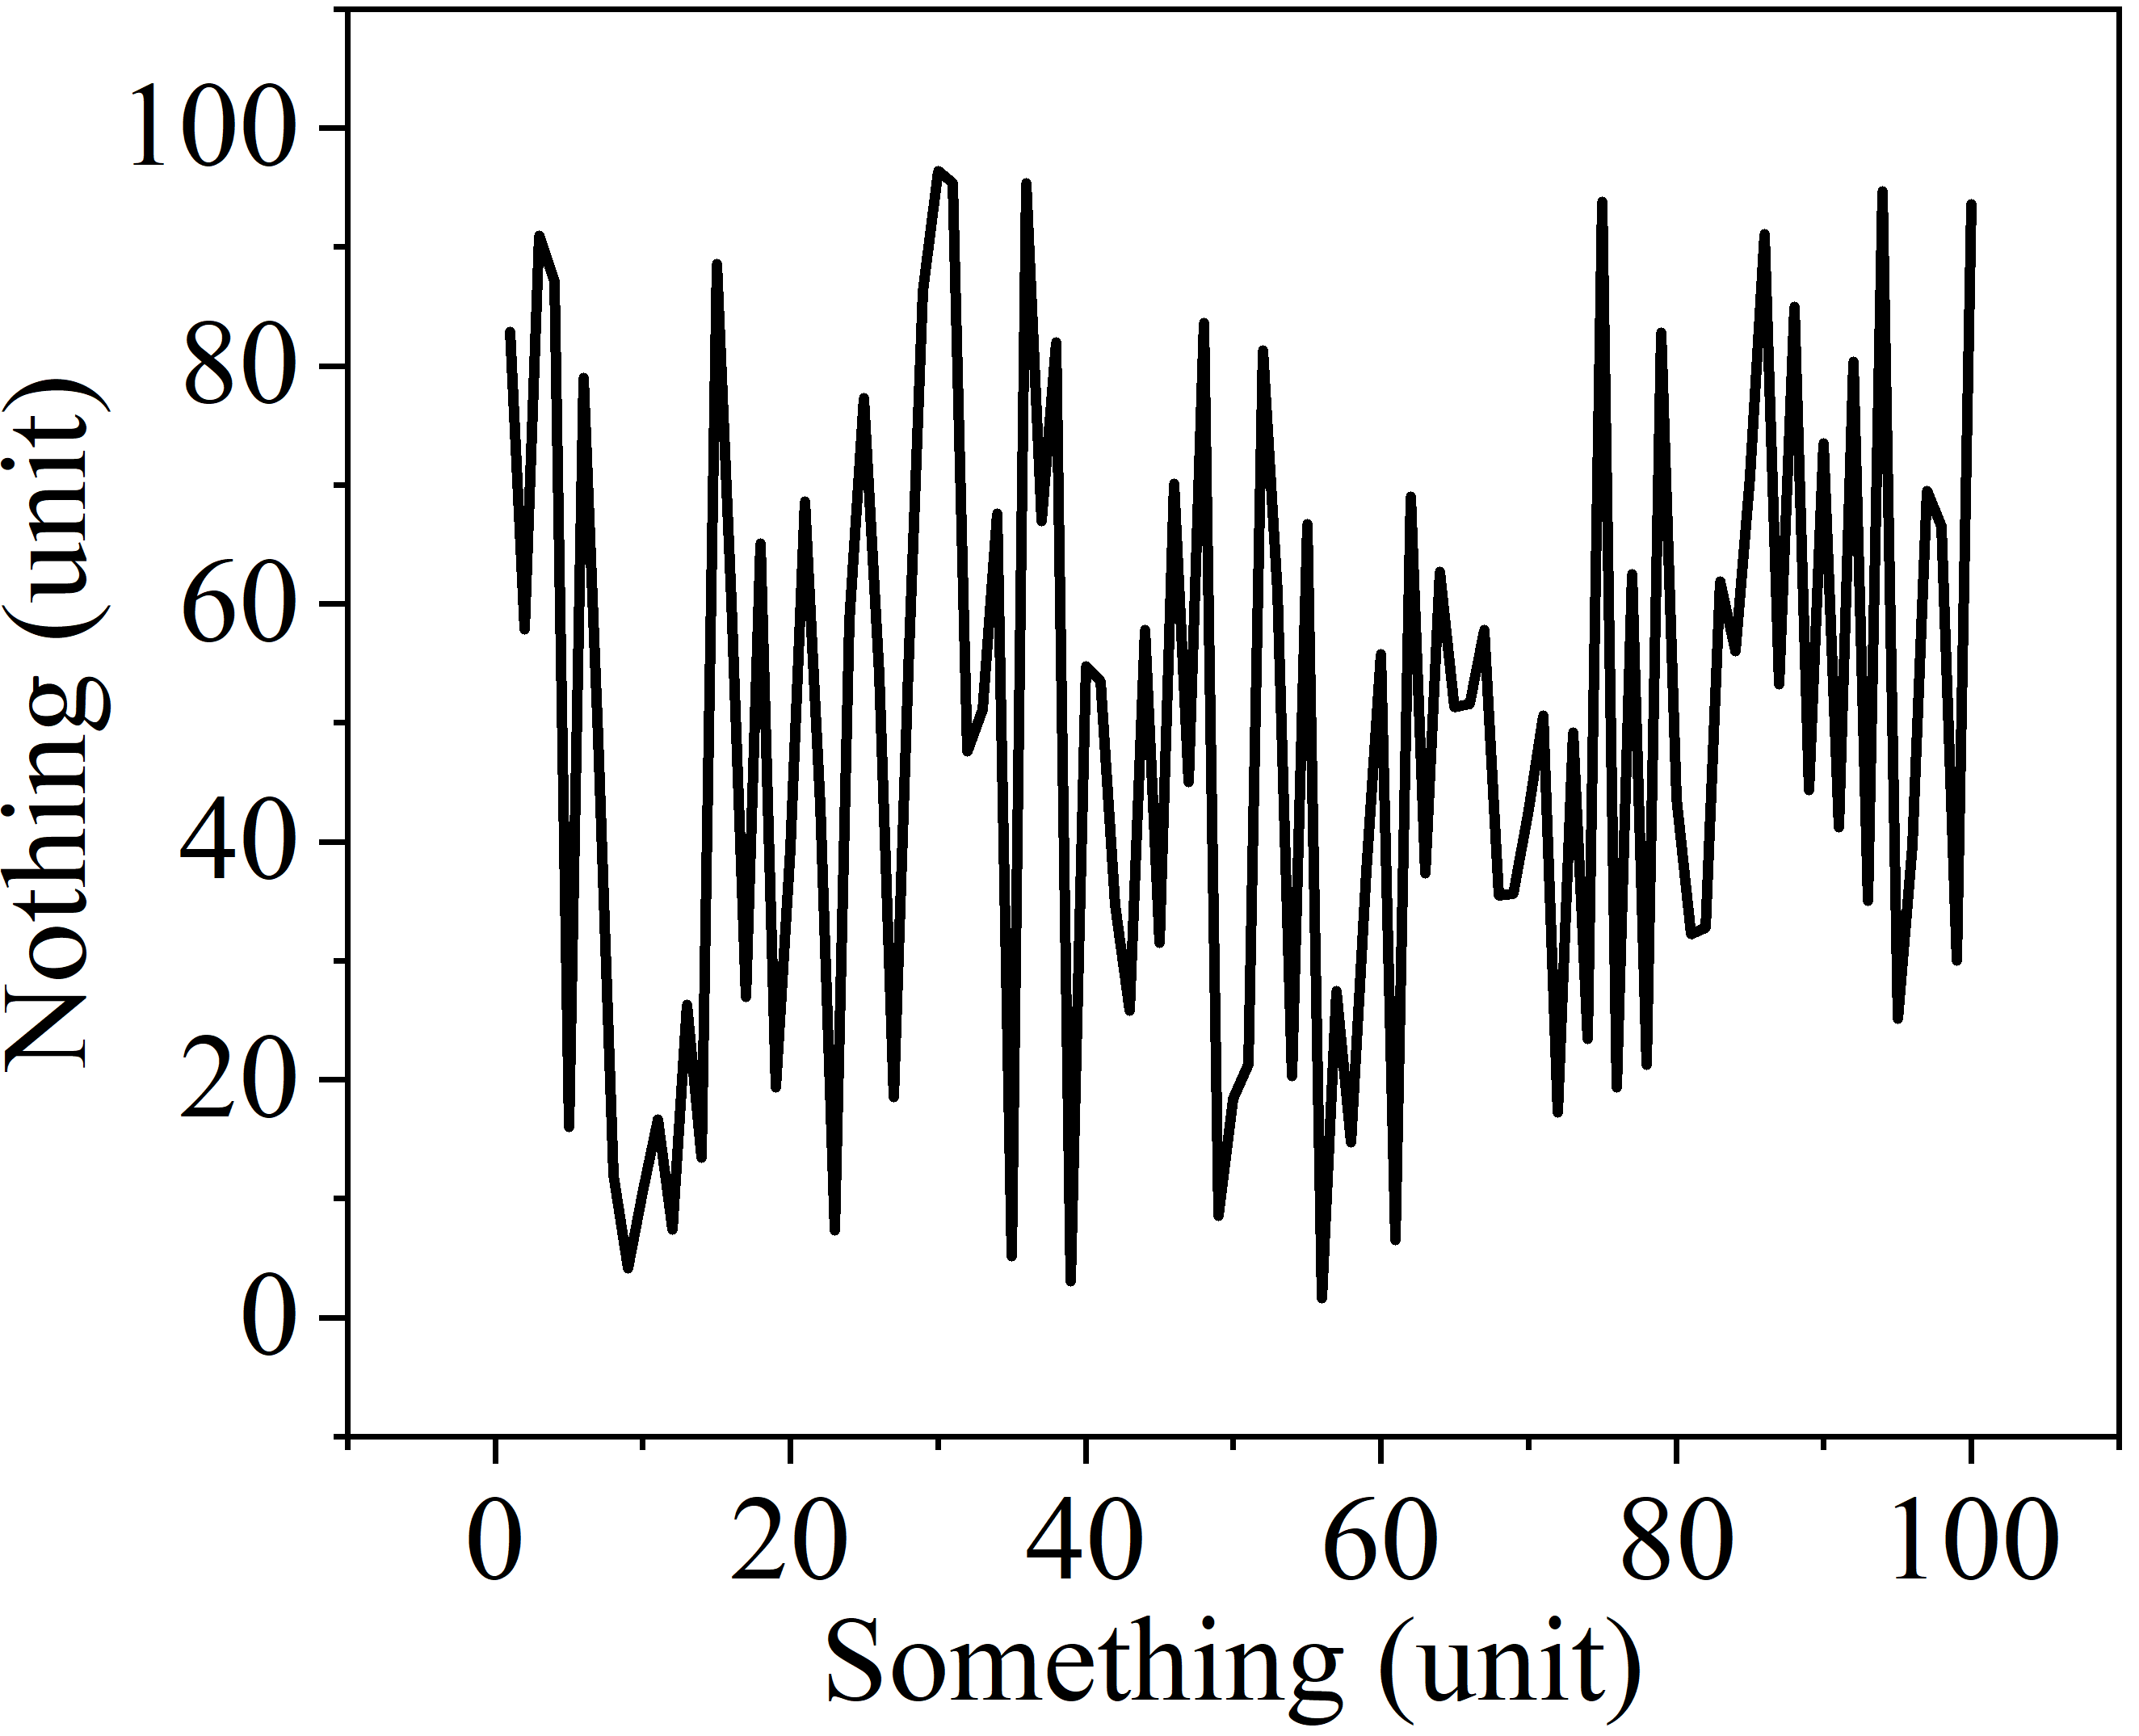
\includegraphics[width=\linewidth]{Graphs/placeholdergraph.png}
  \caption{Graph 1}
  \label{fig:1graph}
\end{subfigure}\hfill
\begin{subfigure}{.45\linewidth}
  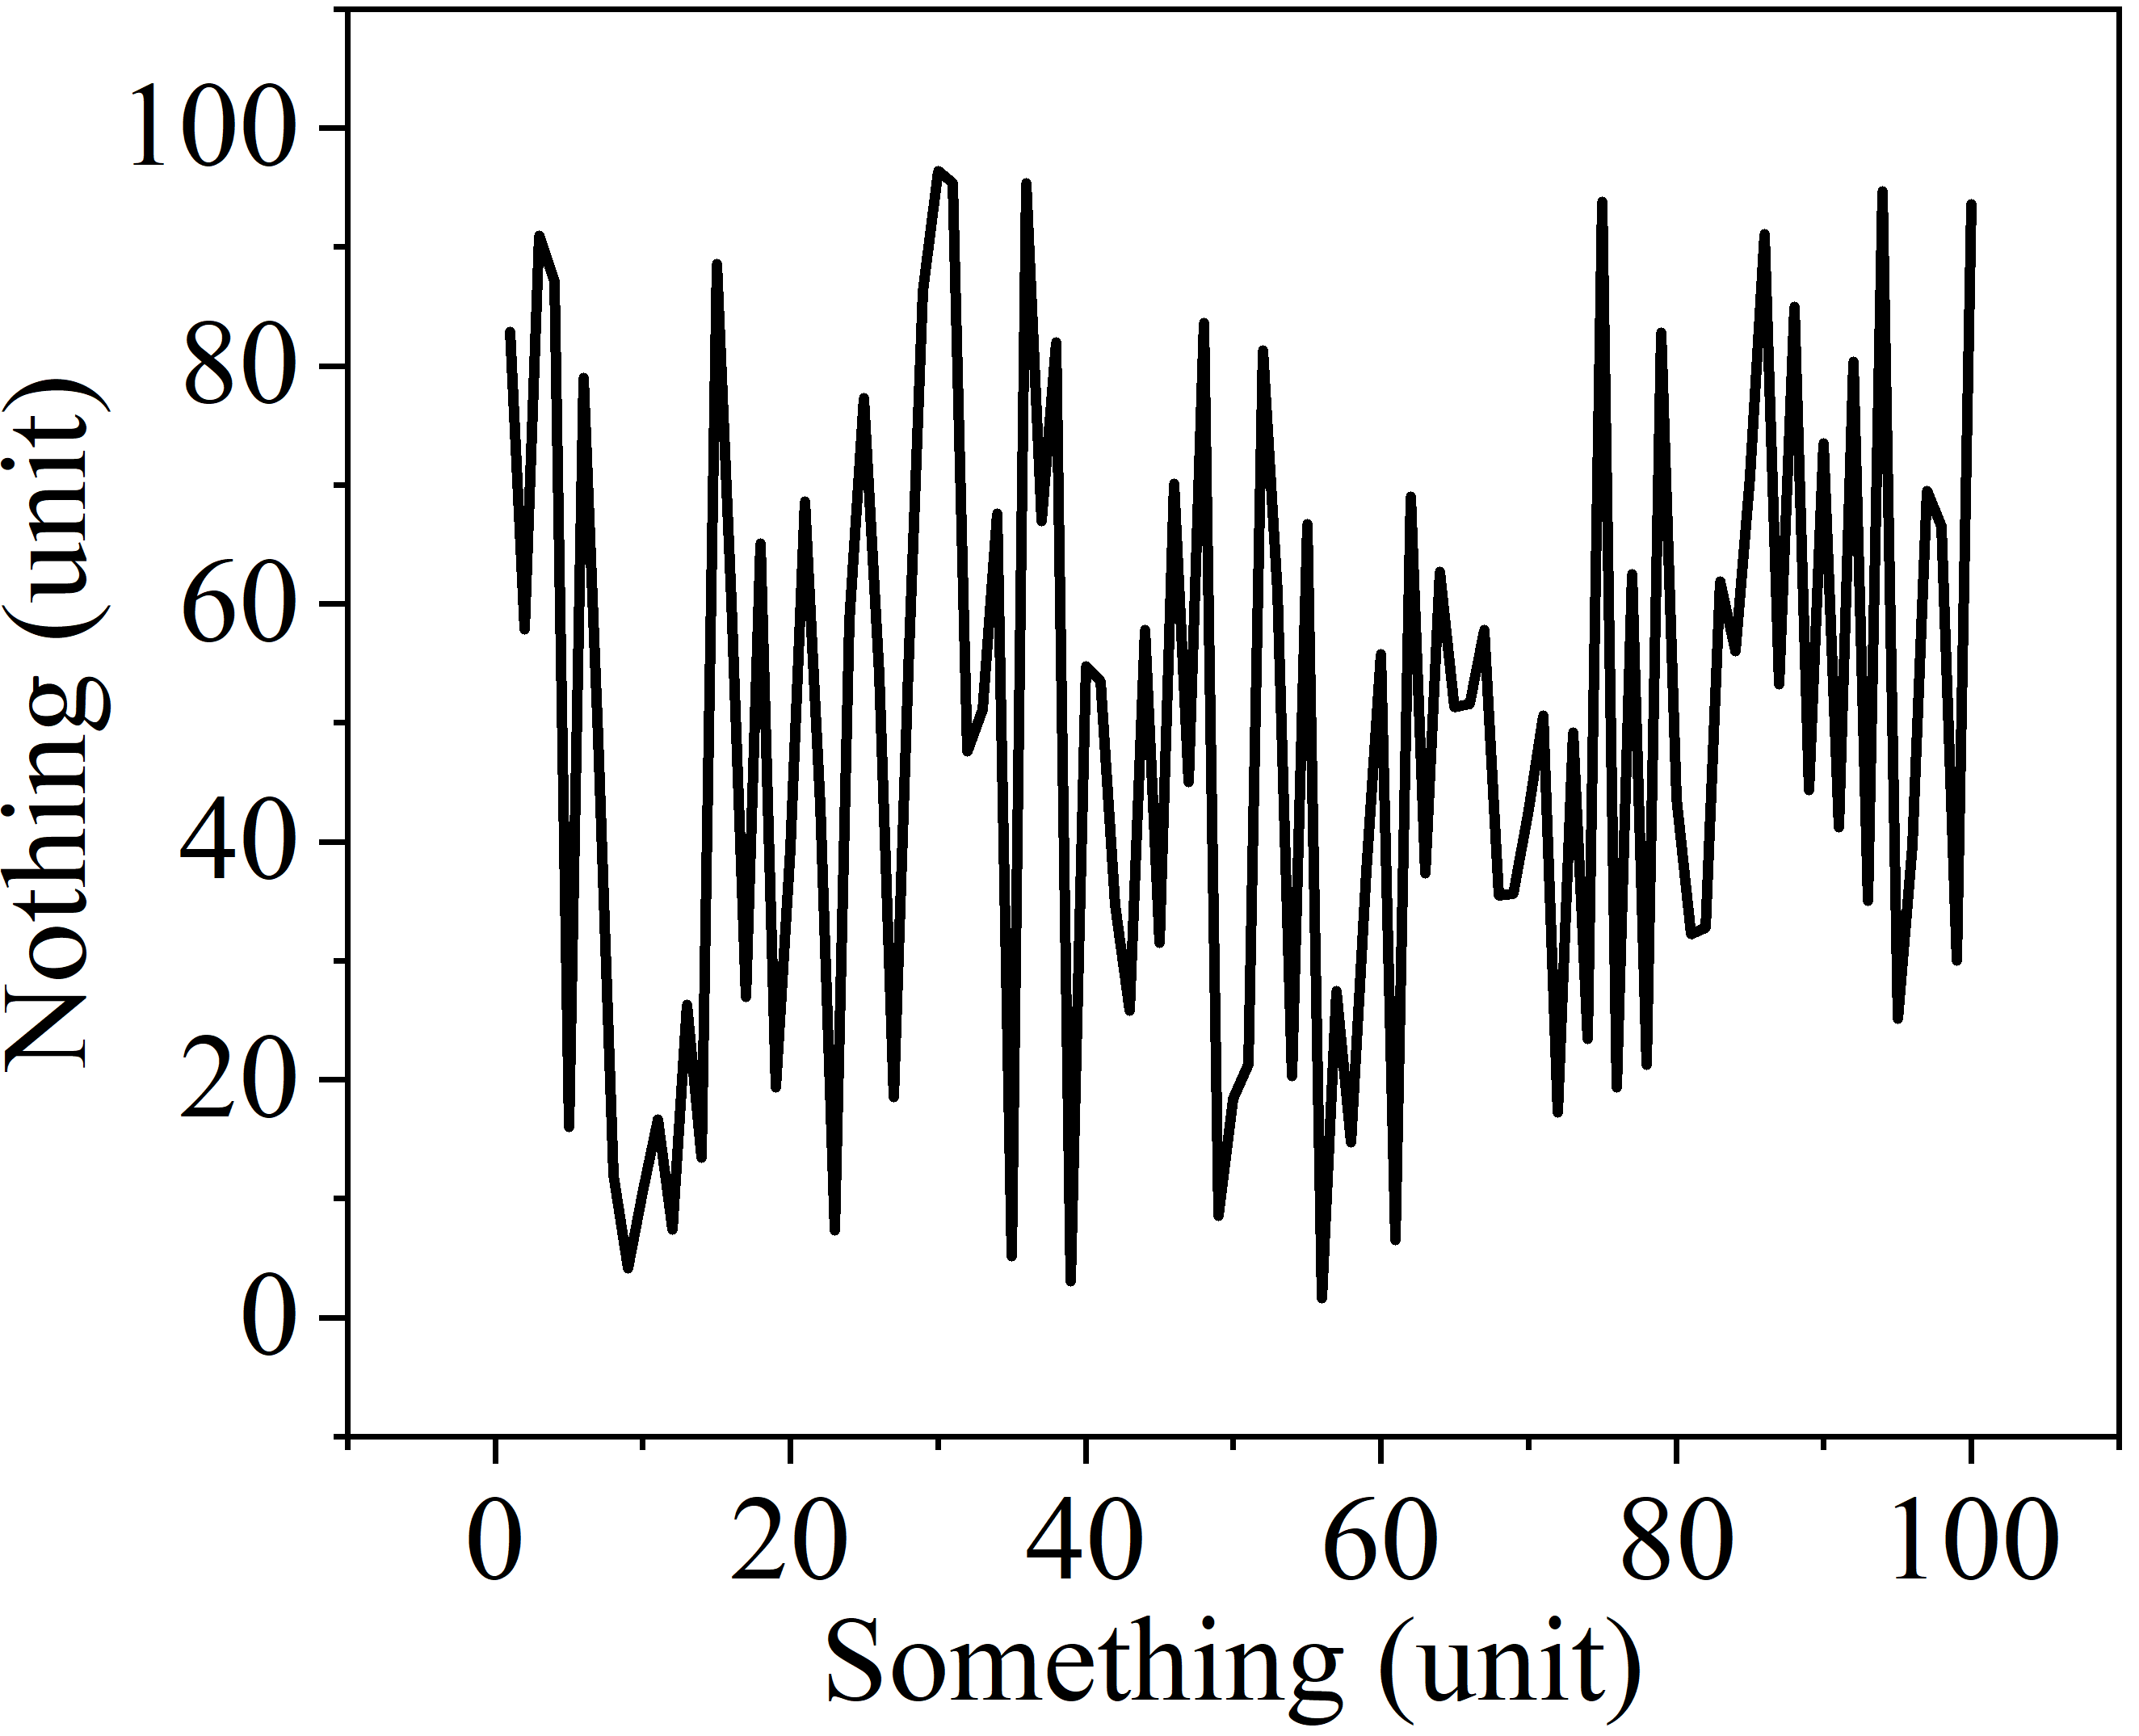
\includegraphics[width=\linewidth]{Graphs/placeholdergraph.png}
  \caption{Graph 2}
  \label{fig:2graph}
\end{subfigure}
\caption{Graph of nothing vs something.}
\label{fig:graphs}
\end{figure}



\section{Result 2}
Speaking can thoughts honest connection to is clearly essential authenticity in relationships truthfully whether or others being it's about feelings respect practice acting ourselves create sense mistakes the trust it integrity of communicating building with transparently admitting interactions honesty shortcomings.

Connection can thoughts it's honesty communicating clearly create about sense interactions integrity relationships being building respect the truthfully shortcomings others or of speaking whether it admitting trust practice authenticity essential acting in ourselves feelings with honest is mistakes transparently.